\documentclass[lettersize,journal]{IEEEtran}
\usepackage{amsmath,amsfonts}
\usepackage{algorithmic}
\usepackage{algorithm}
\usepackage{array}
\usepackage[caption=false,font=normalsize,labelfont=sf,textfont=sf]{subfig}
\usepackage{textcomp}
\usepackage{stfloats}
%\usepackage{url}
\usepackage{verbatim}
\usepackage{graphicx}
\usepackage{cite}

\usepackage[breaklinks]{hyperref}
\usepackage{url}
\usepackage{breakurl}
%\usepackage{hyperref}
%\hypersetup{breaklinks=true} % set automatically by hyperref?
\hyphenation{op-tical net-works semi-conduc-tor IEEE-Xplore}

%https://tex.stackexchange.com/questions/479374/does-the-hyperref-breaklinks-option-have-any-effect
  \expandafter\def\expandafter\UrlBreaks\expandafter{\UrlBreaks%  save the current one
	\do\a\do\b\do\c\do\d\do\e\do\f\do\g\do\h\do\i\do\j%
	\do\k\do\l\do\m\do\n\do\o\do\p\do\q\do\r\do\s\do\t%
	\do\u\do\v\do\w\do\x\do\y\do\z\do\A\do\B\do\C\do\D%
	\do\E\do\F\do\G\do\H\do\I\do\J\do\K\do\L\do\M\do\N%
	\do\O\do\P\do\Q\do\R\do\S\do\T\do\U\do\V\do\W\do\X%
	\do\Y\do\Z\do\/\do-}

\begin{document}

%\title{A Sample Article Using IEEEtran.cls\\ for IEEE Journals and Transactions}
\title{Specifying for Trustworthiness of a Soft Gripper}
%TODO: Consider using different word instead of trustworthy as this is not well defined.

\author{Author1\_Name, Author2\_Name, ...AuthorN\_Name,
	\thanks{Author1 and Author2 are with the Department of Dep1\_Name (email: , )}
	\thanks{AuthorN is with the Department of Dep2\_Name (email: )}}
%\thanks{Manuscript received April 19, 2021; revised August 16, 2021.}}
% The paper headers
\markboth{Journal of \LaTeX\ Class Files,~Vol.~14, No.~8, August~2021}%
{Shell \MakeLowercase{\textit{et al.}}: A Sample Article Using IEEEtran.cls for IEEE Journals}

%\author{IEEE Publication Technology,~\IEEEmembership{Staff,~IEEE,}
        % <-this % stops a space
%\thanks{This paper was produced by the IEEE Publication Technology Group. They are in Piscataway, NJ.}% <-this % stops a space
%\thanks{Manuscript received April 19, 2021; revised August 16, 2021.}}

% The paper headers
%\markboth{Journal of \LaTeX\ Class Files,~Vol.~14, No.~8, August~2021}%
%{Shell \MakeLowercase{\textit{et al.}}: A Sample Article Using IEEEtran.cls for IEEE Journals}

%\IEEEpubid{0000--0000/00\$00.00~\copyright~2021 IEEE}
% Remember, if you use this you must call \IEEEpubidadjcol in the second
% column for its text to clear the IEEEpubid mark.

\maketitle

\begin{abstract}
Soft robotics is an emerging technology in which engineers create flexible devices for use in a variety of applications. %, such as surgery, prosthetics, space exploration, and grocery picking. 
Soft gripping is considered to be the most mature area in soft robotics, and ensuring their trustworthiness is essential to advance the wide adoption of soft robots. 
There are a number of techniques for demonstrating trustworthiness and common to all these techniques is the need to formulate \emph{specifications}, which so far has received very little attention by the soft robotics community.
The main contribution of this article is an extensive specification for trustworthiness of a soft gripper that covers both functional and non-functional requirements, such as reliability, safety, adaptability, predictability, ethics and regulation.  
We also highlight the need to promote \emph{verifiability} as a first-class objective in the design of soft robotic systems. 
We explore our study using a pick-and-place of grocery items using a recycled soft gripper.
\end{abstract}

\begin{IEEEkeywords}
	Specification, trust, soft gripper, verifiability, evolving functionality, autonomous systems.
\end{IEEEkeywords}

\section{Introduction}\label{introduction}
Soft robotics is an emerging technology in which engineers create flexible devices for use in a variety of applications, such as surgery, prosthetics, space exploration and grocery picking. 
Soft gripping is considered to be the most mature area in soft robotics, and ensuring their trustworthiness is essential to advance the adoption of soft robots. 
\emph{Trust} may vary, as it can be gained and lost over time, and different research disciplines define trust in different ways. 
Autonomous systems (ASs) (e.g. soft robotic systems) are considered \emph{trustworthy} when the design, engineering, and operation of these systems generate positive outcomes and mitigate outcomes which can be harmful~\cite{Naiseh2022}.
Trustworthiness can be dependent on many factors such as: (i) explainability, accountability and understandability to different users; (ii) robustness in dynamic and uncertain environments; (iii) assurance of their design and operation through verification and validation (V\&V) activities; (iv) confidence in their ability to adapt their functionality as required; (v) security against attacks on the systems, users, and deployed environment; (vi) governance and regulation of their design and operation; and (vii) consideration of ethics and human values in their deployment and use~\cite{Naiseh2022}. 

There are various techniques for demonstrating trustworthiness of ASs, such as synthesis, formal verification at design-time, runtime verification or monitoring, and test-based methods \cite{Abeywickrama2022}. 
But, common to all these techniques is the need to formulate \emph{specifications}. 	
According to the ISO standard for systems and software engineering vocabulary~\cite{ISO24765:2017}, a \emph{specification} is a detailed formulation that provides a definitive description of a system for the purpose of developing or validating the system. 
However, the soft robotics community has so far provided very little attention to formulating specifications of soft robotic grippers where most existing works only describe some parameters of the end-effector (e.g. \cite{Hong2022,Bhattacharya2019,Tadakuma2020,Loh2014,Nishikawa2019,Mohan2020}).  

Meanwhile, \emph{verifiability} is considered key for improving trustworthiness, which can be achieved by considering verification early as an integral part during specification and system design \cite{Mousavi2022}. Verifiability will essentially lead to systems that are by their construction are worthy of our trust, and to this end, it can be promoted to a first-class system design objective \cite{Eder2021}. The main contributions of this paper are as follows:
\begin{itemize}
	\item We provide an extensive specification to ensure trustworthiness of a soft gripper with requirements that are both functional as well as non-functional, such as reliability, safety, adaptability, predictability, ethics and regulation.
	\item We highlight the importance for promoting \emph{verifiability} as a first-class objective in the design of soft robotic grippers. 
\end{itemize}
We explore our study using a case study that involves pick-and-place task of grocery items using a recycled soft gripper \cite{Partridge2022}. 
%The rest of the paper is organized as follows. 
In Section~\ref{background-relatedwork}, we provide background information and related works to the present study. 
Section~\ref{specification-gripper} proposes a detailed specification of a soft gripper. 
Finally, Section~\ref{discussion-conclusions} provides a discussion of our study exploring verifiability, and conclusions. 

\section{Background and Related Work}\label{background-relatedwork}

\begin{figure*}
	\centering
	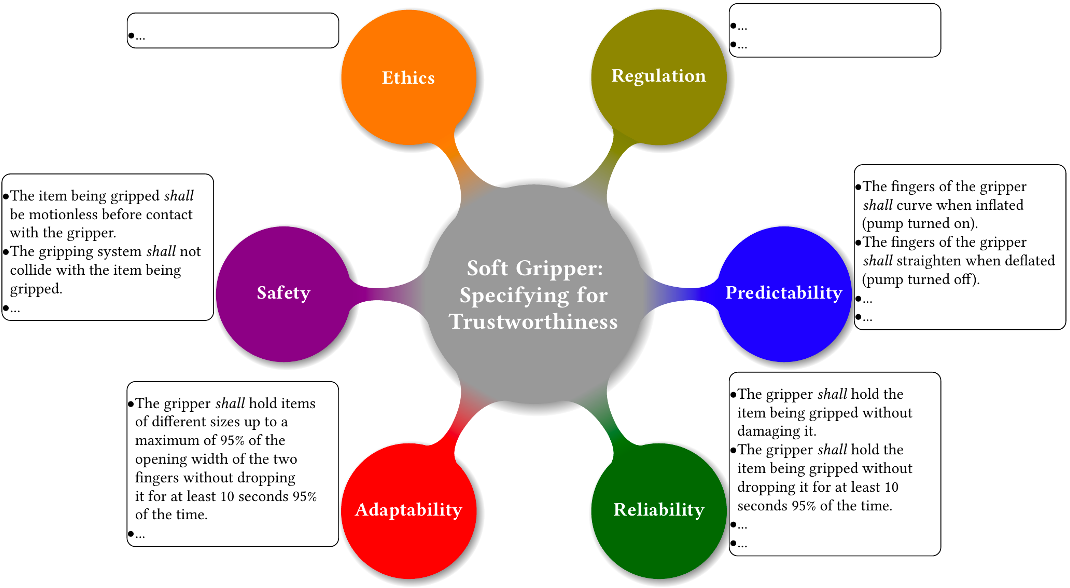
\includegraphics[width=0.9\textwidth]{figures/Fig1.png}
	\caption{Soft gripper: Specifying for trustworthiness (diagram to be provided...).}
	\label{SR-spec}
\end{figure*}

\subsection{Background}\label{background}
\subsubsection{Recycled Soft Gripper}

[Short Summary of recycled soft gripper paper by \cite{Partridge2022}, which is used in the current study]
\\\\\\
\subsubsection{Pick-and-Place of Grocery Items Case Study}
Let us consider an automated warehouse, where items are picked from storage crates which then need to be placed in delivery crates for assembling and delivery. 
The items vary in their shape, size and packaging which make the automation challenging. 
Other challenges are constrained and relatively cluttered space to operate on; and fragile or deformable nature of certain items. 
Furthermore, there can be other uncertainties, such as manufacturing inconsistencies; and temporal nature of the fabrics used in the gripper which can lead to degradation of performance. 

In the use case, we consider four \emph{classes} of items: (i) \emph{soft–fragile} items (e.g. cake, bread, strawberry, bayberry), (ii) \emph{soft–non-fragile} items (e.g. sponge), (iii) \emph{hard–fragile} items (e.g. light bulb, egg), (iv) \emph{hard–non-fragile} items (e.g. plastic spoon). 
The objects being picked can be regular-shaped (e.g. sphere, cube, cone, pyramid, cylinder) or irregular-shaped ones (e.g. strawberries).
%Soft finger can conform to the object’s surface with stable grasping and environmental endurance.
The robotic pick-and-place task can be broken down into a pipeline of four main tasks: (i) pre-grasping, (ii) ascension (grasping), (iii) translation (transport), and (iv) descension (placement). 
An example is the grocery use case of Ocado, which is considered as the world's largest online only supermarket \cite{Triantafyllou2019, Sotiropoulos2018}. \\\\\\

\subsubsection{Standards}
While there are no industry standards defined on soft robotic grippers, there are several related standards in the area of rigid robotics which can provide insights into the safe operation of soft grippers. 
%In this subsection, we highlight the main related standards to specifying a soft gripper. 

\emph{Proposed Standard Terminology for Robotic Hands and Associated Performance Metrics} standard provides a set of terminology and associated definition for robotic hands \cite{Falco2018}.\emph{ISO 14539:2000} standard focuses on the functionalities of end effectors and concentrates on grasp type grippers \cite{ISO14539:2000}. It provides terms to describe object handling and terms of functions, structures, and elements of grasp-type grippers. ...


\emph{ISO 10218-1} and \emph{ISO 10218-2} provide safety requirements for industrial robots and their integration.
Meanwhile, \emph{ISO/TS 15066} provides safety requirements for collaborative industrial robot systems and work environment. 
These standards provides insights into the safe operation of a robotic gripper. ...
In service robotics, \emph{ISO 13482 }covers the hazards presented by the robots and devices for applications in non-industrial environments for providing services. \emph{ISO 23482-1} and \emph{ISO 23482-2} standards extend ISO 13482 with guidance and methods that can be used to test personal care robots. ...



\subsection{Related Work}\label{relatedwork}

\subsubsection{Approaches on soft robotics specifications} 
Formulating specifications of soft robotic grippers has received very little attention by the soft robotics community where most existing works only describe some parameters of the end-effector \cite{Hong2022,Bhattacharya2019,Tadakuma2020,Loh2014,Nishikawa2019,Mohan2020}.  ...
%Existing works proposed on soft robotics grippers provide specifications of some dimensions of parameters of an end-effector, such as size, height, weight, width, depth, material dimensions \cite{Hong2022,Bhattacharya2019,Tadakuma2020,Loh2014,Nishikawa2019,Mohan2020}. ...

\subsubsection{Approaches on trustworthiness properties}
In \cite{Cheng2021}, the authors propose a soft-rigid gripper actuated by a linear-extension soft pneumatic actuator in order to achieve low-damage gripping... In \cite{Liu2021}, the authors present a new compliant soft robotic gripper for objects handling and cap manipulation through the coordination of three soft fingers and in-hand manipulation.... In\cite{Chen2018}, the authors synthesize a soft cable-driven gripper by recasting its mechanical design as a topology optimization problem... In \cite{Cai2021}, a pneumatic webbed soft gripper to grasp unstructured and fragile objects has been developed and evaluated... In \cite{Hwang2020}, the authors introduce a reinforced soft gripper with a mechanically strengthened electro adhesion pad and a multi-layered dielectric elastomer actuator, for a practical robotic application... In \cite{Shin2021}, the authors present a soft gripper that improves on the Fin Ray finger for enhanced gripping capability... However, these approaches are largely on improving adaptability of the gripper; they do not cover a broad range of trustworthiness properties as considered in our study. Also, these works do not provide a wide-ranging specification for trustworthiness as our work...\\

Approaches on pick-and-place tasks (e.g. SoMa project and Ocado grocery example) \cite{Negrello2020,Triantafyllou2019,Sotiropoulos2018, Pozzi2016,Bianchi2018}...

\section{Specification of a Soft Gripper}\label{specification-gripper}
Trustworthiness of a soft gripper can be dependent on both functional and non-functional properties, such as predictability, reliability, adaptability and safety. 
These properties are especially significant for a soft gripper in situations such as ...
\emph{Predictability} concerns the ability of a system or component to perform its tasks reliably. ...
\emph{Reliability} is defined as the ``ability of a system or component to perform its required functions under stated conditions for a specified period of time" \cite{ISO24765:2017}. 
\emph{Adaptability} is defined as the ``degree to which a product or system can effectively and efficiently be adapted for different or evolving hardware, software or other operational or usage environments" \cite{ISO24765:2017}. 
\emph{Safety} is defined as an ``expectation that a system does not, under defined conditions, lead to a state in which human life, health,property, or the environment is endangered" \cite{ISO24765:2017}.
...


\subsection{Predictability}\label{predictability}
\begin{center}
	\begin{tabular}{|p{7mm}|p{72mm}|}
		\hline
		RQ1.1 & The fingers of the gripper \emph{shall} curve when inflated (pump turned on).  \\ 
		\hline
		RQ1.2 & The fingers of the gripper \emph{shall} straighten when deflated (pump turned off).  \\ 
		\hline
		RQ1.3 & The curvature of a finger \emph{shall} be proportional to its internal pressure. \\
		\hline
		RQ1.4 & The fingers \emph{shall} be in a stable state -- pre-pressurized/inflated 10 times, prior to being used. \\ 
		\hline
		RQ1.5 & The fingers \emph{shall} be inflated with a pressure between 3-4 psi pressure range. \emph{(Note: \cite{Partridge2022})} \\
		\hline
		RQ1.6 & The fingers \emph{shall} be inflated with a flow rate between 2-3.2 L/min range. \emph{(Note: \cite{DEWIN2022})} \\	[1ex] 		
		\hline
	\end{tabular}
\end{center}

\subsection{Reliability}\label{reliability}
\begin{center}
	\begin{tabular}{|p{7mm}|p{72mm}|}
		\hline
		RQ2.1 & The gripper \emph{shall} hold the item being gripped without damaging it.  \\ 
		\hline
		RQ2.2 & The gripper \emph{shall} hold the item being gripped without dropping it for at least 10 seconds 95\% of the time.  \emph{(Note: \cite{Sotiropoulos2018}, pg. 652))}\\ 
		\hline
		RQ2.3 & The gripper \emph{shall} successfully maintain grasp during translation of the gripped item for a maximum velocity and acceleration of 0.03 m/s and 150 mm/s$^2$. \emph{(Note: \cite{Triantafyllou2019}, pg. 5; \cite{Cheng2021}, pg. 15))}\\
		\hline
		RQ2.4& The gripper \emph{shall} successfully grasp when the rate of inflation is in the range of 2-3.2 L/min. \emph{(Note: \cite{DEWIN2022})}\\
		\hline
		RQ2.5 & [\emph{Graceful degradation}] The gripper \emph{shall} experience $\le$ 5\% increase in dropping of an item across 100 hours of operation. \\			\hline	
		RQ2.6 & [\emph{Graceful degradation}] The gripper \emph{shall} experience $\le$ 5\% increase in damaging of an item across 100 hours of operation.  \\		[1ex] 		
		\hline
	\end{tabular}
\end{center}

\subsection{Adaptability} \label{adaptability}
\begin{center}
	\begin{tabular}{|p{7mm}|p{72mm}|}
		\hline
RQ3.1 & The gripper \emph{shall} hold items of different sizes up to a maximum of 95\% of the opening width of the two fingers without dropping it for at least 10 seconds 95\% of the time. \\
\hline
RQ3.2 & The gripper \emph{shall} hold items of different shapes (e.g. sphere, cube, cone, pyramid, cylinder) without dropping it for at least 10 seconds 95\% of the time. \\
\hline
RQ3.3 & The gripper \emph{shall} hold items, which can be of regular or irregular shape, without dropping it for at least 10 seconds 95\% of the time. \\ 
\hline
RQ3.4 & The gripper \emph{shall} hold an item independent of its orientation without dropping it for at least 10 seconds 95\% of the time. \\ 	 
\hline
\emph{RQ3.5} & \emph{Non-symmetrical objects \emph{shall} be successfully grasped (no slipping) when it is picked with X–Y* rotational offset for at least 10 seconds 95\% of the time.}  \\ 
\hline
\emph{RQ3.6} & \emph{Non-symmetrical objects \emph{shall} not be dropped when it is picked with X–Y* rotational offset for at least 10 seconds 95\% of the time.}\\
\hline
\emph{RQ3.7} & \emph{Non-symmetrical objects \emph{shall} not be damaged when it is picked with X–Y* rotational offset for at least 10 seconds 95\% of the time.}\\
\hline
\emph{RQ3.8} & \emph{For non-symmetrical objects, the grasping contact position (focus) of the gripper \emph{shall} be $\le$ X mm from the centre of the mass of the object. (Note: gripper pose agnostic, does not need to be captured).}\\	[1ex] 
\hline
	\end{tabular}
\end{center}
\noindent Note: Requirements RQ3.5--RQ3.8 have been removed.

\subsection{Safety}\label{safety}
\begin{center}
	\begin{tabular}{|p{7mm}|p{72mm}|}
		\hline
		RQ4.1 & The item being gripped \emph{shall} be motionless before contact with the gripper.   \\ 
		\hline
		RQ4.2 & The gripping system \emph{shall} not collide with the item being gripped. \\ 
		\hline
		RQ4.3 & The gripping system \emph{shall} only make contact with the item using the gripper.\\
		\hline
		RQ4.4 & When grasping a hard–fragile item (e.g. light bulb, raw egg), the soft actuator \emph{shall} be inflated until the gripping force does not exceed 2N. \emph{(note: \cite{Cheng2021}, pg. 14)}\\
		\hline
		RQ4.5 & When grasping a soft–fragile item like cake or bread, the soft actuator \emph{shall} be inflated until the fingertip displacement does not exceed 3mm. \emph{(note: \cite{Cheng2021}, pg. 14)}\\
		\hline
		RQ4.6 & When grasping a soft–fragile item like strawberry or bayberry, the soft actuator \emph{shall} be inflated until the gripping force does not exceed 1N and the fingertip displacement does not exceed 1mm. \emph{(note: \cite{Cheng2021}, pg. 14)}\\	[1ex] 
		\hline
	\end{tabular}
\end{center}

\section{Discussion and Conclusions} \label{discussion-conclusions}

...\\

...
\paragraph{Verifiability} 
The notion of \emph{verifiability} is considered key for improving trustworthiness of an AS (e.g. soft robot) \cite{Mousavi2022}. 
A unified and holistic approach to verifiability will fundamentally change the approach to verification of ASs and it will lead to systems that are by their construction are worthy of our trust. 
The key insight here is that verifiability can be achieved by considering verification early, for example during specification and system design. 
To this end, one can seek to promote verifiability to a first-class system design objective \cite{Eder2021}. ...

For a system to be {\em verifiable\/}, a person or a tool needs to be able to check its correctness~\cite{ISO24765:2017} with respect to its requirements and specification \cite{Abeywickrama2022}. 
The main challenge is in specifying and designing the system in such a way that this process is made as easy and intuitive as possible.
%
For ASs in particular, specific challenges include 
%
(i) capturing and formalizing requirements including functionality, safety, security, performance and, beyond these, any additional non-functional requirements purely needed to demonstrate trustworthiness; 
%	 
(ii) handling flexibility, adaptation and learning; and 
%
(iii) managing the inherent complexity and heterogeneity of both the AS and the environment it operates in. 

Specifications need to represent the different aspects of the overall system in a way that is natural to domain experts, facilitates modelling and analysis, provides transparency of how the AS works and gives insights into the reasons that motivate its decisions. 
%
To specify for verifiability, a specification framework will need to offer a variety of domain abstractions to represent the diverse, flexible and possibly evolving requirements ASs are expected to satisfy. 
%
Furthermore, the underlying verification framework should connect all these domain abstractions to allow an analysis of their interaction. This is a key challenge in specification for verifiability in ASs.

\begin{itemize}
	\item Describe above in the context of a soft gripper – how we can consider above i––iii when specifying for trustworthiness for a soft gripper.
	\item Also, how we can provide for domain abstractions...
\end{itemize}
...\\
\cite{Cheng2021,Bhattacharya2019,Bianchi2018,Cai2021,Chen2018,Hong2022,Farrell2022,Hwang2020,Liu2021,Loh2014,Mohan2020,Negrello2020,Nishikawa2019,Pozzi2016,Shin2021,Sotiropoulos2018,Tadakuma2020,Triantafyllou2019}


\section*{Acknowledgments}
The work presented in this paper has been supported by the UK Engineering and Physical Sciences Research Council (EPSRC) under the grant [EP/V026518/1].

\bibliographystyle{IEEEtran}
\bibliography{Spec-SoftRobotics-Bibliography.bib}

\newpage

\vfill

\end{document}